\appendix

\section{Reproducing our work}
% \begin{lstlisting}
% go get git.torproject.org/user/phw/sybilhunter.git
% \end{lstlisting}
Redacted for anonymization.

\section{Mathematical metric}
\label{sec:metric}
The following conditions have to be met in order to classify as a mathematical
metric.  While points 1, 2, and 3 are typically straightforward to satisfy,
point 4, the triangle inequality, can turn out to be tricky.
\begin{enumerate}
	\item $d(x, y) \geq 0$
	\item $d(x, y) = 0$ iff $x = y$
	\item $d(x, y) = d(y, x)$
	\item $d(x, z) \leq d(x, y) + d(y, z)$
\end{enumerate}

\section{Supporting diagrams}

\begin{figure}[t]
	\centering
	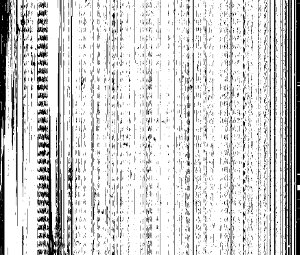
\includegraphics[width=\linewidth]{diagrams/default-sybils-2015-10.jpg}
	\caption{Uptimes for ``default'' Sybils in Oct. 2015.  Many relays exhibit a
	diurnal pattern, suggesting that the relays }
	\label{fig:default-sybils-uptime}
\end{figure}
